\documentclass[tikz,border=4mm]{standalone}
\usepackage{amsmath,amssymb}
\usepackage{tikz}
\usetikzlibrary{arrows.meta,positioning,shapes.geometric,shapes.misc,fit,backgrounds,decorations.pathreplacing,shadows,calc}

% Professional Academic Color Palette (Nature / NeurIPS style)
\definecolor{seqblue}{RGB}{24, 76, 120}
\definecolor{seqbluebg}{RGB}{242, 247, 252}
\definecolor{timecyan}{RGB}{14, 116, 144}
\definecolor{timecyanbg}{RGB}{236, 254, 255}
\definecolor{ontoviolet}{RGB}{79, 70, 229}
\definecolor{ontovioletbg}{RGB}{245, 243, 255}
\definecolor{lawgreen}{RGB}{22, 101, 52}
\definecolor{lawgreenbg}{RGB}{240, 253, 244}
\definecolor{alertred}{RGB}{190, 18, 60}
\definecolor{alertredbg}{RGB}{255, 241, 242}
\definecolor{boxborder}{RGB}{148, 163, 184}
\definecolor{darkslate}{RGB}{30, 41, 59}

\begin{document}
\begin{tikzpicture}[
    font=\sffamily,
    >=Stealth,
    node distance=1.0cm,
    card/.style={
        draw=boxborder!70,
        fill=white,
        rounded corners=4pt,
        drop shadow={opacity=0.10, shadow xshift=1.2pt, shadow yshift=-1.2pt},
        inner sep=6pt
    },
    module/.style={
        draw=#1!80!black,
        fill=#1bg,
        rounded corners=4pt,
        drop shadow={opacity=0.08, shadow xshift=1.2pt, shadow yshift=-1.2pt},
        inner sep=6pt
    },
    tag/.style={
        fill=#1,
        text=white,
        font=\sffamily\bfseries\tiny,
        rounded corners=2pt,
        inner sep=2.5pt
    },
    arrowlabel/.style={
        font=\sffamily\tiny,
        fill=white,
        inner sep=1.5pt,
        text=darkslate
    }
]

% ==============================================================================
% STAGE 1: DYNAMIC CIVIL CASE & TEMPORAL INTERACTION GRAPH
% ==============================================================================
\node[card, text width=4.3cm] (casecard) {
    {\color{seqblue}\textbf{\small 1. Legal Case Fact Sequence}}\\[2pt]
    \rule{4.3cm}{0.4pt}\\[3pt]
    \scriptsize
    \textbf{Claimant $u$ (Buyer)} $\leftrightarrow$ \textbf{Respondent $v$ (Seller)}\\[3pt]
    $\bullet$ \textbf{$t_0$ (2020-01-15):} Deposit Contract ($500$M VND)\\
    $\bullet$ \textbf{$t_1$ (2020-03-01):} Default \& Notice of Breach\\
    $\bullet$ \textbf{$t_2$ (2023-06-20):} Lawsuit filed ($\Delta t = 1,254$\,d)\\[3pt]
    \rule{4.3cm}{0.4pt}\\[2pt]
    \tiny\color{alertred}\textbf{Event Stream:} $\mathcal{S}_{\text{case}} = \{(u, v, r_i, t_i)\}_{i=1}^M$
};
\node[tag=seqblue, above=1pt of casecard.north west, anchor=south west] {STAGE I: EPISODIC INPUT};

\node[card, below=0.6cm of casecard, text width=4.3cm, align=center] (graphnode) {
    {\color{seqblue}\textbf{\small Dynamic Interaction Graph $\mathcal{G}(t)$}}\\[5pt]
    \begin{tikzpicture}[scale=0.9]
        \node[circle, draw=seqblue, fill=seqblue!15, inner sep=3pt, font=\scriptsize\bfseries] (u) at (0, 0) {$u$};
        \node[circle, draw=seqblue, fill=seqblue!15, inner sep=3pt, font=\scriptsize\bfseries] (v) at (3.2, 0) {$v$};
        \draw[->, thick, color=seqblue] (u) to[bend left=25] node[above, font=\tiny] {$e_{1}, t_0$ (Deposit)} (v);
        \draw[->, thick, color=alertred] (v) to[bend left=25] node[below, font=\tiny] {$e_{2}, t_1$ (Breach)} (u);
        \node[draw=gray!50, dashed, rounded corners=2pt, fill=gray!5, inner sep=2pt, font=\tiny] at (1.6, -1.0) {$\Delta t = t_2 - t_1 = 1,254$\,days};
    \end{tikzpicture}
};

\node[draw=seqblue!40, dashed, rounded corners=6pt, fill=seqbluebg!30, fit=(casecard)(graphnode), inner sep=8pt] (stage1box) {};

% ==============================================================================
% STAGE 2: CONTINUOUS HARMONIC ENCODING & AXIOM-TGAT
% ==============================================================================
\node[module=timecyan, right=1.2cm of casecard.north east, anchor=north west, text width=4.5cm] (bochner) {
    {\color{timecyan}\textbf{\small Bochner Continuous Time Kernel}}\\[2pt]
    \rule{4.5cm}{0.4pt}\\[3pt]
    \scriptsize
    $\Phi(\Delta t) = \frac{1}{\sqrt{d_{\tau}}} \left[\cos(\boldsymbol{\omega} \Delta t)^\top \parallel \sin(\boldsymbol{\omega} \Delta t)^\top\right]^\top$\\[2pt]
    \tiny Continuous Fourier Embedding ($\boldsymbol{\omega}_k \sim \mathcal{N}(0, \sigma^2)$)\\[4pt]
    \centering
    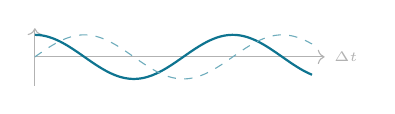
\begin{tikzpicture}[xscale=0.4, yscale=0.28]
        \draw[->, gray!60] (0,0) -- (9.2,0) node[right, font=\tiny] {$\Delta t$};
        \draw[->, gray!60] (0,-1.3) -- (0,1.3);
        \draw[domain=0:8.8, samples=60, smooth, thick, color=timecyan] plot (\x, {cos(\x*180/3.14159)});
        \draw[domain=0:8.8, samples=60, smooth, dashed, color=timecyan!60] plot (\x, {sin(\x*180/3.14159)});
    \end{tikzpicture}
};
\node[tag=timecyan, above=1pt of bochner.north west, anchor=south west] {CONTINUOUS TIME EMBEDDING};

\node[module=seqblue, below=0.6cm of bochner, text width=4.5cm] (tgat) {
    {\color{seqblue}\textbf{\small Axiom-TGAT Message Passing ($\times L$)}}\\[2pt]
    \rule{4.5cm}{0.4pt}\\[3pt]
    \scriptsize
    \textbf{Temporal Attention Weights:}\\
    $\alpha_{uv}^{(l)} = \operatorname{Softmax}_v \left(\frac{(\mathbf{h}_u \mathbf{W}_Q)(\mathbf{h}_v \parallel \mathbf{e}_{uv} \parallel \Phi(\Delta t))^\top \mathbf{W}_K^\top}{\sqrt{d}}\right)$\\[4pt]
    \textbf{Aggregation \& Skip Residual $\bigoplus$:}\\
    $\widetilde{\mathbf{h}}_u^{(l)} = \sum_{v \in \mathcal{N}_u} \alpha_{uv}^{(l)} (\mathbf{h}_v \parallel \mathbf{e}_{uv} \parallel \Phi(\Delta t)) \mathbf{W}_V$\\
    $\mathbf{h}_u^{(l)} = \operatorname{LayerNorm}\left(\mathbf{h}_u^{(l-1)} + \widetilde{\mathbf{h}}_u^{(l)}\right)$\\[3pt]
    \tiny\centering\color{seqblue}\textbf{Dynamic Node States:} $\mathbf{z}_{uv}(t) = [\mathbf{h}_u^{(L)}(t) \parallel \mathbf{h}_v^{(L)}(t)]$
};
\node[tag=seqblue, above=1pt of tgat.north west, anchor=south west] {STAGE II: TEMPORAL GNN};

\node[draw=timecyan!50, dashed, rounded corners=6pt, fill=timecyanbg!20, fit=(bochner)(tgat), inner sep=8pt] (stage2box) {};

% ==============================================================================
% STAGE 3: TBOX STATUTORY AXIOMS & HERMIT REASONER
% ==============================================================================
\node[module=ontoviolet, right=1.2cm of bochner.north east, anchor=north west, text width=4.6cm] (tbox) {
    {\color{ontoviolet}\textbf{\small OWL 2 DL Formal Ontology $\mathcal{O}_{\text{civil}}$}}\\[2pt]
    \rule{4.6cm}{0.4pt}\\[3pt]
    \scriptsize
    \textbf{TBox Statutory Axioms ($\mathcal{SROIQ}$):}\\
    $\bullet$ $\text{Valid} \sqcap \text{Void} \sqsubseteq \bot$ \hfill \tiny(Disjointness)\\[2pt]
    $\bullet$ $\text{Voidable} \sqcap \exists \text{curedBy}.(\text{Perform} \ge \frac{2}{3}) \sqsubseteq \text{Valid}$\\
    \null\hfill \tiny(Art. 129(2) Curing)\\[2pt]
    $\bullet$ $\text{Claim} \sqcap \exists \Delta t > 3\,\text{years} \sqsubseteq \text{TimeBarred}$\\
    \null\hfill \tiny(Art. 429 Prescription Bar)\\[3pt]
    \rule{4.6cm}{0.4pt}\\[2pt]
    \textbf{Automated Hypertableau Reasoner:}\\
    $\bullet$ Provable Consistency: $\mathcal{O}_{\text{civil}} \cup \mathcal{A}_{\text{case}} \not\models \bot$\\
    $\bullet$ Penalty: $\mathcal{L}_{\text{onto}} = \sum_{a \in \mathcal{A}_{\text{viol}}} \max(0, -\log P(a))$
};
\node[tag=ontoviolet, above=1pt of tbox.north west, anchor=south west] {STAGE III: TBOX GUARDRAIL};

\node[module=alertred, below=0.6cm of tbox, text width=4.6cm] (statepred) {
    {\color{alertred}\textbf{\small 4-State Automaton Predictor}}\\[2pt]
    \rule{4.6cm}{0.4pt}\\[3pt]
    \scriptsize
    $\mathbf{p}_{\text{state}}(t) = \operatorname{Softmax}(\mathbf{W}_s \mathbf{z}_{uv}(t) + \mathbf{b}_s) \in \Delta^4$\\[3pt]
    States: $\{S_0: \text{Valid}, S_1: \text{Voidable},$\\
    \phantom{States: } $S_2: \text{Void}, S_3: \text{Extinguished}\}$\\[3pt]
    \rule{4.6cm}{0.4pt}\\[2pt]
    \tiny\color{darkslate}\textbf{Total Loss:} $\mathcal{L} = \mathcal{L}_{\text{CE}} + \lambda_{\text{trans}} \mathcal{L}_{\text{trans}} + \lambda_{\text{onto}} \mathcal{L}_{\text{onto}}$
};
\node[tag=alertred, above=1pt of statepred.north west, anchor=south west] {NEURAL PREDICTION};

\node[draw=ontoviolet!50, dashed, rounded corners=6pt, fill=ontovioletbg!20, fit=(tbox)(statepred), inner sep=8pt] (stage3box) {};

% ==============================================================================
% STAGE 4: DEFEASIBLE DUNG FRAMEWORK & ADJUDICATION VERDICT
% ==============================================================================
\node[module=lawgreen, right=1.2cm of tbox.north east, anchor=north west, text width=4.0cm] (dung) {
    {\color{lawgreen}\textbf{\small Defeasible Framework $AF$}}\\[2pt]
    \rule{4.0cm}{0.4pt}\\[3pt]
    \scriptsize
    $AF = \langle \mathcal{A}, \mathcal{R}_{\text{defeat}} \rangle$\\[4pt]
    \centering
    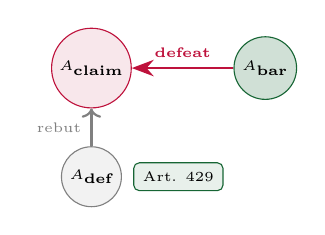
\begin{tikzpicture}[scale=0.92]
        \node[circle, draw=alertred, fill=alertred!10, inner sep=2pt, font=\tiny\bfseries] (aclaim) at (0, 0.9) {$A_{\text{claim}}$};
        \node[circle, draw=gray, fill=gray!10, inner sep=2pt, font=\tiny\bfseries] (adef) at (0, -0.6) {$A_{\text{def}}$};
        \node[circle, draw=lawgreen, fill=lawgreen!20, inner sep=2pt, font=\tiny\bfseries] (abar) at (2.4, 0.9) {$A_{\text{bar}}$};
        
        \draw[->, thick, color=gray] (adef) -- node[left, font=\tiny] {rebut} (aclaim);
        \draw[->, thick, color=alertred, -{Stealth[scale=1.2]}] (abar) -- node[above, font=\tiny\bfseries] {defeat} (aclaim);
        \node[draw=lawgreen, fill=lawgreen!10, rounded corners=2pt, font=\tiny] at (1.2, -0.6) {Art. 429};
    \end{tikzpicture}\\[3pt]
    \rule{4.0cm}{0.4pt}\\[2pt]
    \tiny
    \textbf{Knaster-Tarski Least Fixed Point:}\\
    $GE(AF) = \operatorname{lfp}(F_{AF}) = \{A_{\text{bar}}\}$
};
\node[tag=lawgreen, above=1pt of dung.north west, anchor=south west] {STAGE IV: DEFEASIBLE DUNG HEAD};

\node[card, below=0.6cm of dung, text width=4.0cm, draw=lawgreen!80!black, fill=lawgreenbg] (verdict) {
    \centering
    {\color{lawgreen}\textbf{\small Certified Judicial Decree}}\\[2pt]
    \rule{4.0cm}{0.4pt}\\[3pt]
    \scriptsize
    \textbf{Adjudication Outcome:}\\[2pt]
    \textbf{\color{alertred}\normalsize ACTION DISMISSED}\\[2pt]
    \tiny
    Statute of Limitations Expired\\
    ($\Delta t = 1,254 > 1,095$\,days, Art. 429)\\[3pt]
    \rule{4.0cm}{0.4pt}\\[2pt]
    \scriptsize\color{lawgreen}\textbf{Verification Status:}\\
    $\checkmark$ 100\% TBox Axiom Compliance\\
    $\checkmark$ Grounded Defeasible Proof
};
\node[tag=lawgreen, above=1pt of verdict.north west, anchor=south west] {CERTIFIED VERDICT};

\node[draw=lawgreen!50, dashed, rounded corners=6pt, fill=lawgreenbg!20, fit=(dung)(verdict), inner sep=8pt] (stage4box) {};

% ==============================================================================
% INTER-STAGE CONNECTIONS & DATA FLOW PIPELINE
% ==============================================================================
\draw[->, very thick, color=seqblue] (casecard.east) -- node[above, arrowlabel] {$\{(u,v,r_i,t_i)\}$} (tgat.west);
\draw[->, very thick, color=timecyan] (graphnode.east) -| ++(0.5, 0) |- node[above, arrowlabel, pos=0.7] {$\Delta t$} (bochner.west);
\draw[->, very thick, color=timecyan] (bochner.south) -- node[right, arrowlabel] {$\Phi(\Delta t)$} (tgat.north);

\draw[->, very thick, color=seqblue] (tgat.east) -- node[above, arrowlabel] {$\mathbf{z}_{uv}(t)$} (statepred.west);
\draw[->, very thick, color=seqblue] (tgat.east) -| ++(0.5, 0) |- node[above, arrowlabel, pos=0.7] {ABox Assertions} (tbox.west);
\draw[<->, thick, dashed, color=ontoviolet] (tbox.south) -- node[right, arrowlabel] {$\mathcal{L}_{\text{onto}}$ Guardrail} (statepred.north);

\draw[->, very thick, color=ontoviolet] (tbox.east) -- node[above, arrowlabel] {$\mathcal{A}_{\text{just}}$} (dung.west);
\draw[->, very thick, color=alertred] (statepred.east) -| ++(0.5, 0) |- node[above, arrowlabel, pos=0.7] {$\mathbf{p}_{\text{state}}$} (verdict.west);
\draw[->, very thick, color=lawgreen] (dung.south) -- node[right, arrowlabel] {$GE(AF)$} (verdict.north);

\end{tikzpicture}
\end{document}
